\documentclass{article}
\usepackage{graphicx} % Required for inserting images
\usepackage[colorlinks=true, allcolors=blue]{hyperref}
\usepackage[square,numbers]{natbib}
\usepackage{titlesec}
\usepackage{geometry}
 \geometry{
 a4paper,
 total={170mm,257mm},
 left=20mm,
 top=20mm,
 }
\graphicspath{ {./images/} }

\title{Unit 23}
\author{Chris}
\date{}
\bibliographystyle{abbrvnat}

\begin{document}

\section{How cognitive computing can be used to help improve business activities}

\section{Healthcare}
According to a recent review published in PubMed "Cognitive computing, is an evolving technology in healthcare augments the clinical thought process and enable the doctors to make the right diagnosis and preserve the patient's health in good condition."\cite{pubmed}. These healthcare systems can provide timely care, optimal and cost-effective treatment according to this meta review. Highlighting the platforms, techniques, tools, algorithms, applications, and use case. 
There are already a number of cognitive platforms in the area of health including
\begin{itemize}
    \item IBM Watson
    \item Microsoft Cortana Intelligence Suite
    \item Google Deepmind
    \item SparkCognition’s SparkPredict
    \item Expert System’s Cogito
    \item Numenta’s NuPIC
    \item CognitiveScale’s Cognitive Cloud
    \item HealthTap’s Dr. AI
    \item Enterra solution’s Aila
    \item Healthcare X.0’s Cognitive Assist
\end{itemize}



\section{Retail}
Cognitive computing has revolutionized the way enterprises operate and make decisions. By leveraging advanced technologies such as Artificial Intelligence (AI) and Machine Learning (ML), businesses can now harness the power of cognitive computing to streamline processes, enhance customer experiences, and gain valuable insights. Large Language Models (LLM) and Natural Language Processing (NLP) have revolutionized many use cases, enhancing productivity and experience. 

\section{Education}
The interactions between education and industry are a remarkable feature of cognitive computing, especially when it comes to its applications in education and learning. For example, companies like IBM are using cognitive computing to harness the power of Big Data in multiple areas, including education.
According to Gartner, "The global market for AI in education is projected to reach \$6.1 billion by 2025." /cite{emb} and "72\% of educational institutions are investing in AI-driven technologies to enhance learning outcomes".
There specifically are huge benefits to using LLMs in eduction 
\begin{itemize}
    \item Personalized learning - Customize learning experiences for each student
    \item Automated tasks - Grading etc
    \item New and innovative educational tools and resources - LLMs can be used to create interactive simulations, games
    \item Real-time feedback and support - Chat bots can provide quick help and feedback to students
\end{itemize} \cite{packtpub}

\section{Finance}
Cognitive computing helps fiance by improving client-facing services, future innovations and feasibility studies on innovation opportunities. How client-facing can improve with cognitive computer are doing provide innovative financial advisory solutions that would enable them to better serve their customers, and give them an edge in their competitive industry. How future innovations can improve with cognitive computing is by helping the client to understand the technology forecast and where best to use them and when it is ready to be used.
Chatbots specifically can give
\begin{itemize}
    \item Detailed customer analysis
    \item Contextualized customer service
    \item Improved security and identity management - by analuyzing customer behaviors
\end{itemize} \cite{pulse}

\section{Diagrams}
Diagram of cognitive computer in healthcare \\
\includegraphics[scale=0.5]{Healthcare} \\
Diagram of cognitive computing \\
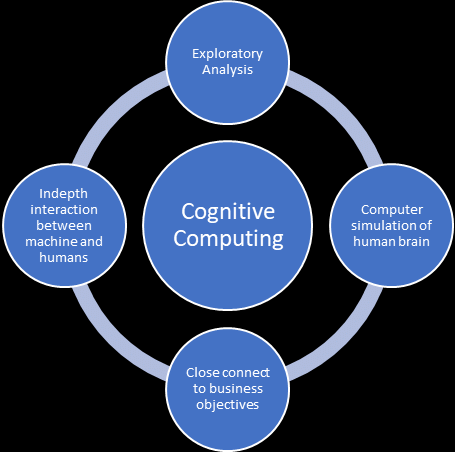
\includegraphics[scale=0.5]{Cognitive} \\

\break
\bibliography{bibliography}

\end{document}
